\documentclass[a4paper,10pt]{article}
%\documentclass[a4paper,10pt]{scrartcl}

\usepackage[utf8]{inputenc}
\usepackage[german]{babel}
\usepackage[pdftex]{graphicx}
\usepackage{listings}
\usepackage{color}
\usepackage{amssymb}
\usepackage{marvosym}
\usepackage{amsmath}
\usepackage{array}
\usepackage{geometry}
\usepackage{listings}
\usepackage{upgreek}
\usepackage{color}
\usepackage{gensymb}

\geometry{verbose,tmargin=2cm,bmargin=2cm,lmargin=2cm,rmargin=2.5cm,headheight=80pt}
\newcolumntype{L}[1]{>{\raggedright\arraybackslash}p{#1}} % linksbündig mit Breitenangabe
\newcolumntype{C}[1]{>{\centering\arraybackslash}p{#1}} % zentriert mit Breitenangabe
\newcolumntype{R}[1]{>{\raggedleft\arraybackslash}p{#1}} % rechtsbündig mit Breitenangabe

\newcommand{\f}{\textbf}
\newcommand{\ku}{\textit}
\newcommand{\zb}{z.B.\ }
\newcommand{\ia}{i.A.\ }
\newcommand{\ua}{u.a.\ }
\newcommand{\idr}{i.d.R.\ }

\title{SSD}
\author{}
\date{}

\pdfinfo{%
  /Title    ()
  /Author   ()
  /Creator  ()
  /Producer ()
  /Subject  ()
  /Keywords ()
}

\begin{document}
\maketitle

\section{Spacecraft System Design}
\f{Mission concept:} 
\begin{itemize}
 \item subject (what for)
 \item orbit and constellation
 \item payload, bus
 \item launch element
 \item ground element
 \item mission operations
 \item command, communication, control
\end{itemize}
\begin{figure}[ht!]
 \centering
 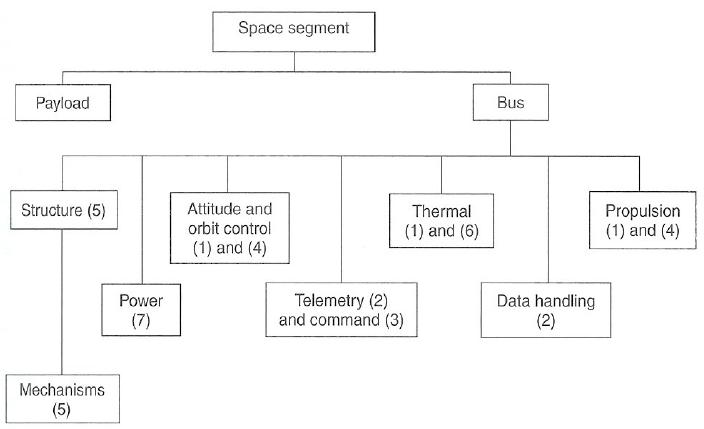
\includegraphics[scale=0.6]{overview}
\end{figure}

\section{Space Dynamics/Kepler Orbits}
\f{Typical coordinate systems:}
\begin{itemize}
 \item spacecraft-fixed
 \begin{itemize}
  \item Mittelpunkt des Satelliten = Ursprung
  \item nadir = z-Achse, nominale Geschwindigkeit = x-Achse
  \item gut, um Position und Orientierung der Satelliteninstrumente festzustellen
 \end{itemize}
 \item earth-fixed 
 \begin{itemize}
  \item Mittelpunkt der Erde = Ursprung
  \item durch greenwich meridian = x-Achse
  \item Geolocation, Satellitenbewegung
 \end{itemize}
 \item roll, pitch and yaw-coordinates 
 \item celestial coordinates
 \begin{itemize}
  \item Mittelpunkt der Erde = Ursprung
  \item Richtung Frühlingspunkt = x-Achse
  \item Orbitanalyse, Astronomie
 \end{itemize}
\end{itemize}
\f{Keplergesetze}
\begin{enumerate}
 \item der Orbit eines jeden Planeten ist eine Ellipse, wobei die Sonne in einem der Fixpunkte liegt
 \item die Verbindungslinie zwischen Sonne und Planet überstreicht in gleichen Zeiten gleiche Flächen 
 \item die Quadrate der Umlaufzeiten sind proportional zu den Kuben der großen Halbachsen
\end{enumerate}
\f{Ellipsendinge}
\begin{itemize}
 \item a \dots große Halbachse
 \item $\varepsilon$, e \dots Exzentrizität, ``Abplattung'' der Ellipse ($\varepsilon$=0: Kreis, $\varepsilon$=1: Parabel, $0<\varepsilon<1$: Ellipse)
\end{itemize}
\f{Begriffe: }
\begin{itemize}
 \item Periapsis: Punkt der Ellipse, der am nähesten an dem Zentralkörper liegt (bei Sonne: Perihel, bei Erde: Perigäum)
 \item Apoapsis: Punkt der Ellipse, der am weitesten entfernt vom Zentralkörper liegt (bei Sonne: Apohel, bei Erde: Apogäum)
 \item Distanz zu Periapsis $r_p = a(1-\varepsilon)$, Distanz zu Apoapsis $r_a = a(1+\varepsilon)$
\end{itemize}
\f{6 Bahnelemente:}
\vspace*{10pt}

\begin{figure}[!ht]
\begin{minipage}{0.35\textwidth}
 \begin{itemize}
  \item große Halbachse a
  \item Exzentrizität $\varepsilon$
  \item inclination i
  \item right ascension of the ascending node $\Omega$
  \item argument of perigee $\omega$
  \item true anomaly $\nu$
 \end{itemize} 
\end{minipage}
\hfill
\begin{minipage}{0.64\textwidth}
  \centering
  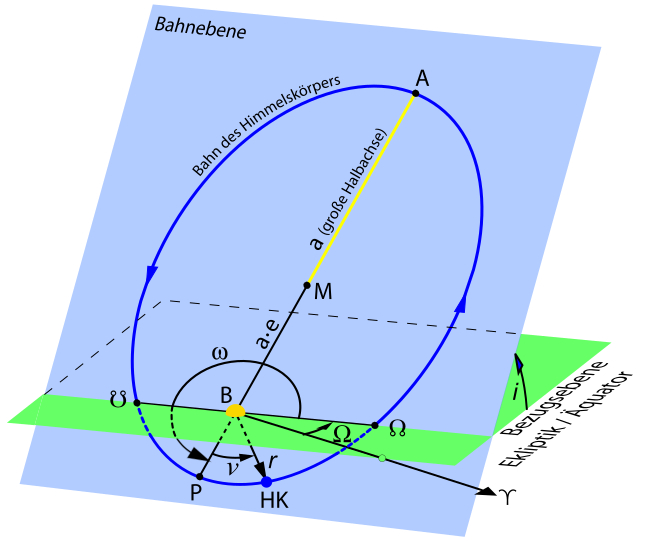
\includegraphics[scale=0.55]{BahnelementeEllipse}
\end{minipage}
\end{figure}
\noindent \f{Lieblingsformel}
\[T = 2\pi\sqrt{\frac{a^3}{\mu}}\]
\f{Change of the right ascension of the ascending node}
\[\Delta \Omega = - \frac{3\pi J_2R_E^2}{a^2(1-\varepsilon^2)^2}cos(i)\]
\f{Change of the argument of perigee}
\[\Delta \omega = \frac{3\pi J_2R_E^2}{2a^2(1-\varepsilon^2)^2}(4-5sin^2(i))\]

\noindent \f{Orbits}
\begin{enumerate}
 \item Highly Elliptical Orbit HEO
 \begin{itemize}
  \item hohe Exzentrizität
  \item große Halbachsen
  \item dadurch lange Kontakdauer zum Satelliten
  \item Werte für Perigäum: 200 bis 15.000 km
  \item Werte für Apogäum: 50.000 bis 140.000 km
  \item für Forschung (\zb Weltraumteleskope), Telekommunikation, Militär 
  \item Beispiel: Molniya-Orbit (feste Inklination von 63,4$^\circ$, Periodendauer von einem halben Sterntag (23h56m4s))
 \end{itemize}
 \item Sun-Synchronous Orbit
 \begin{figure}[!ht]
  \centering
  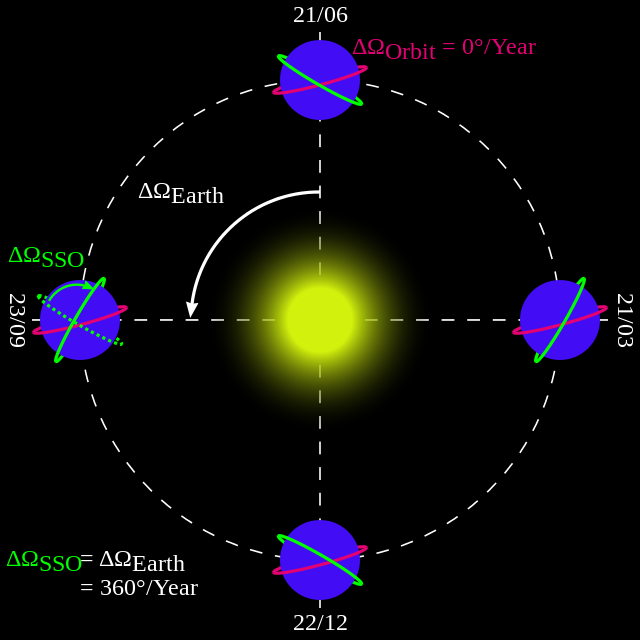
\includegraphics[scale=0.4]{sso}
 \end{figure}
 \begin{itemize}
  \item Höhe und Inklination werden so kombiniert, dass ein Satellite aus Sicht der Sonne immer auf dem selben Orbit ist
  \item Höhe: 600-800 km
  \item Inklination: leicht retrograd ($\approx 98^\circ$)
  \item Umlaufdauer: 96-100min
 \end{itemize}

 \item Geostationary Orbit GEO
 \begin{itemize}
  \item kreisförmiger Orbit
  \item Höhe: 35.786km
  \item Umlaufdauer: 24h
  \item Wettersatelliten, Kommunikationssatelliten, Fernsehsatelliten
 \end{itemize}

\end{enumerate}

\noindent \f{Subsatellite Point} = intersection of the line between satellite and earth center with the earth's surface 
\noindent \f{Hohmann Transfer}
\begin{figure}[!ht]
 \centering
 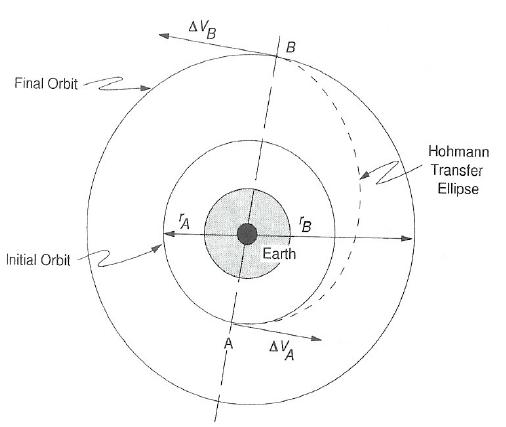
\includegraphics[scale=0.6]{hohmann}
\end{figure}

\begin{itemize}
\item Calculate a transfer between two circular orbits with radius $r_A$ to $r_B$. The velocity at pericenter of the transfer ellipse:
\[ v_P^2 = 2 \mu \left( \frac{1}{r_A} - \frac{1}{r_A + r_B} \right) = 2 \mu \frac{r_B}{r_A(r_A+r_B)} \]
\item The required $\Delta v_A$ to inject from the transfer orbit:
\[ \Delta v_A = v_P - v_A = \sqrt{\frac{\mu}{r_A}} \left( \sqrt{\frac{2r_B}{r_A+r_B}} -1\right) \]
\item The required $\Delta v$ to inject from the transfer orbit into orbit with $r_B$:
\[ \Delta v_B = v_B - v_\text{apo} = \sqrt{\frac{\mu}{r_B}} \left( 1 - \sqrt{\frac{2r_A}{r_A+r_B}}\right) \]
where $v_B$ is the circular velocity at $r_B$.
\item The Hohmann transfer is the most energy-efficient transfer between two circular orbits.
\[ \Delta v_\text{total} =  \Delta v_A + \Delta v_B = \sqrt{\mu}\left[ \sqrt{\left( \frac{2}{r_A} - \frac{2}{r_A+r_B} \right)} - \sqrt{\frac{1}{r_A}} + \sqrt{\frac{2}{r_B}-\frac{2}{r_A+r_B}} - \sqrt{\frac{1}{r_B}} \right]\]
\end{itemize}

\section{Mission Analyses}
\f{Earth-Synchronous Orbit}
\begin{itemize}
 \item the ground track repeats after a specific period of time
 \item Earth's rotation rate is the sidereal rotation period = sidereal day $\uptau_{\text{\tiny{E}}}$
 \item $\uptau_E$ is varying with time $\uptau_E = 86164.10555+0.15\cdot C$ [s] where C is the centuries since year 2000
 \item as the Earth rotates eastward, the satellite is thus moving relative to the surface in westward direction by 
 \[\Delta \Phi_r = 2\pi\frac{T}{\uptau_{\text{\tiny{E}}}} \text{ [rad/rev]}\] 
 \item second effect influencing the shift of the subsatellite point is the rotation of the satellite's orbit plane $\Delta \Omega$
 \item as $\Delta \Omega$ is positive in eastward direction, these two effects are combined to the total angular shift $\Delta \Phi$ at subsequent equator 
 passages \[\Delta \Phi = \Delta \Phi_r - \Delta \Omega \text{ [rad/rev]}\]
 \item to be Earth-Synchronous: 
 \[n\Delta \Phi = m \cdot 2\pi\]
\end{itemize}
\f{Sun-Synchronous Orbit}
\begin{itemize}
 \item die Erde braucht $\uptau_S = 3.155815\cdot 10^7 s$, um einmal um die Sonne zu kreisen 
 \item bei einem sonnensynchronen Orbit muss der Winkel zwischen Sonnenrichtung und Orbitebene konstant bleiben 
 \item also muss sich die Ebene pro Tag um einen Winkel $\theta$ drehen 
 \[\theta = 2\pi\frac{\uptau_{\text{\tiny{E}}}}{\uptau_{\text{\tiny{S}}}} \text{ [rad/day]} = 2\pi\frac{\uptau_{\text{\tiny{E}}}}{\uptau_{\text{\tiny{S}}}}\frac{T}{\uptau_{\text{\tiny{E}}}} \text{ [rad/rev]}\]
\end{itemize}
\f{Earth- and Sun-Synchronous Orbit}
\begin{itemize}
 \item \[\Delta \Omega = \theta \Rightarrow T\left(\frac{1}{\uptau_{\text{\tiny{E}}}} - \frac{1}{\uptau_{\text{\tiny{S}}}}\right) = \frac{m}{n}\]
 \item angular shift between two subsequent orbits 
 \[\Delta \Phi = \Delta \Phi_r - \Delta \Omega = 2\pi T\left(\frac{1}{\uptau_{\text{\tiny{E}}}} - \frac{1}{\uptau_{\text{\tiny{S}}}}\right) \text{ [rad/rev]}\]
 worst case between subsequent orbits $\Delta \Phi \cdot R_E$.
\end{itemize}
\f{Eclipse periods}
angle between Earth-Sun vector and normal vector to orbit plane: $\sin \beta = \vec{s}\cdot\vec{n}$\\
Earth central angular radius at entry into eclipse: $\beta^* = \sin^{-1}\left(\frac{R_E}{h+R_E}\right)$\\
Angular arc of orbit in shadow: $2\cos^{-1}\left(\frac{\cos \beta^*}{\cos \beta}\right)$
\f{Ground Contact and Coverage Analyses}
altitude $h$, visible horizon characterized by angles $\rho$ and $\lambda_0$: $\rho + \lambda_0 = 90\degree$
\begin{align*}
 R_E &= (R_E + h) \cos \lambda_0\\
 &= (R_E +h) \sin \rho\\
\end{align*}
observe $\Lambda_t, \Theta_t$ (long,lat) from known orbit position of satellite, characterized by subsatellite point $\Lambda_s, \Theta_s$.\\
characteristic paramters:
\begin{itemize}
 \item nadir angle $\eta$
 \item earth central angle $\lambda$
 \item spacecraft elevation angle $\varepsilon$
\end{itemize}
\begin{figure}[!ht]
 \centering
 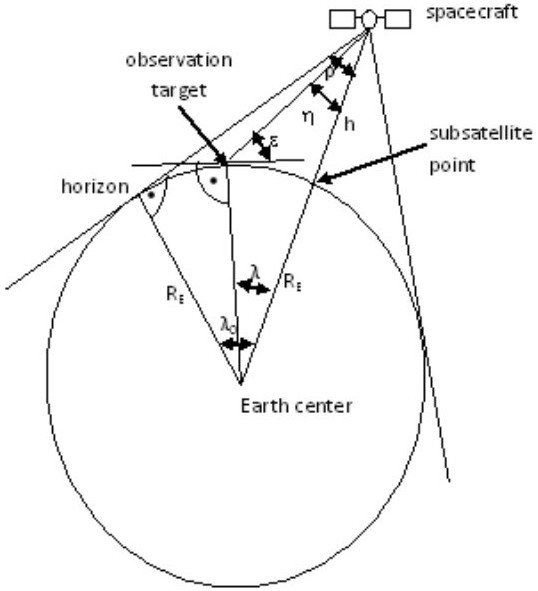
\includegraphics[scale=0.6]{groundcoverage}
\end{figure}
calculate nadir angle $\eta$:
\[ \tan \eta = \frac{\frac{R_E}{R_E+h}\sin \lambda}{1-\frac{R_E}{R_E+h}\cos\lambda}\]
\[ \lambda + \eta + \varepsilon = 90\degree \]
$\lambda_\text{max}$: maximum earth central angle $\Rightarrow$ swath width $2\lambda_\text{max}$ perpendicular to groundtrack on surface.\\
Time in view $T_\text{view}$ for circular orbit with period $T$:
\[ T_\text{view} = \frac{T}{180\degree}\cos^{-1}\left(\frac{\cos \lambda_\text{max}}{\cos \lambda}\right)\]
\f{ground station contact periods}
\begin{figure}[!ht]
 \centering
 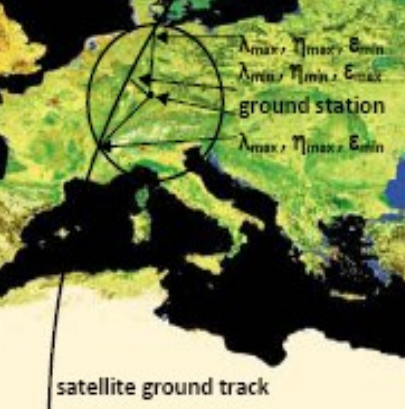
\includegraphics[scale=0.6]{groundtrack}
\end{figure}
\begin{itemize}
 \item $\sin\eta_\text{max} = \cos \varepsilon_\text{min}\frac{R_E}{R_E+h}$
 \item $\lambda_\text{max} = 90\degree - \varepsilon_\text{min} -\eta_\text{max}$
 \item max range satellite$\leftrightarrow$groundstation: $D_\text{max} = R_E\frac{\sin\lambda_\text{max}}{\sin\eta_\text{max}}$
 \item total time in view: $ T_\text{view} = \frac{T}{180\degree}\cos^{-1}\left(\frac{\cos \lambda_\text{max}}{\cos \lambda_\text{min}}\right)$
 \item contact only possible, if station-orbit angle $<$ central angle of contact cone
\end{itemize}

\section{Distributed Satellite Systems}
\begin{itemize}
 \item \f{constellation}: similar trajectories without relative position control.
 \item \f{formation}: closed-loop onboard control for topology in the group.
 \item \f{swarm}: similar vehicles cooperating without fixed positions, selfdetermined.
 \item \f{cluster}: heterogenous system of vehicles for joint objective.
\end{itemize}
requirements on distributed satellite systems: coordination of
\begin{itemize}
 \item orbits at different altitudes
 \item optimal control strategies for position/attitude of components
 \item activities for heterogenous sensors
 \item information flow and storage
\end{itemize}
\f{Walker Delta Pattern Constellation}
\[ i: t/p/f \]
\begin{itemize}
 \item i: inclination
 \item t: total $\sharp$ satellites
 \item p: $\sharp$ equally shaped orbit planes
 \item f: relative phase difference between satellites in adjacent planes
\end{itemize}
Example: Galileo is $56\degree: 27/3/1$ with circular orbits ($h =23222km$), nine satellites always in view, one spare satellite in each plane.
\f{earth surface converage}
$ s = \frac{t}{p}$ number of satellites equally spaced in plane with angular distance $\Delta v = \frac{360\degree}{s}$. There are two cases:
\begin{itemize}
 \item $\Delta v < 2\cdot \lambda_\text{max} \Rightarrow$ area of continuous coverage exists (``street of coverage'')
 \item $\Delta v > 2\cdot \lambda_\text{max} \Rightarrow$ no street of coverage
\end{itemize}
Street-width: $\cos \lambda_\text{street} = \frac{\cos\lambda_\text{max}}{\cos\frac{\Delta v}{2}}$

\f{formation flying arcitectures and dynamics}
\begin{itemize}
 \item \f{virtual structure}: treated as single structure
 \item \f{behavioral strategies}: distributed control approach, following nature.
 \item \f{leader-follower}: divided into leaders and followers. followers track designated leaders with prescribed offset. absolute/relative control architecture.
\end{itemize}

\f{communication in low-earth orbit distributed satellite systems}
\begin{itemize}
 \item comm and tele-operation infrastructure is key element for distributed systems
 \item transfer position and observation data for formation flying
 \item amount of data increases with swarm size
 \item analyse pre-processing procedures, intersatellite links and ground station links
\end{itemize}

\f{conclusion on distributed satellite systems}
\begin{itemize}
 \item research field due to paradigm shift from one large spacecraft to several smaller crafts
 \item higher fault tolerance and robustness
 \item swarms are scaleable
 \item gun launches into orbit
 \item comination of big and small spacecrafts
 \item swarms for survailance and earth observation
 \item LEO $\rightarrow$ high spatial resolution
 \item higher temporal resolution is provided by constellations with several satellites in the same orbit
\end{itemize}








\section{Mechanics}

\section{Thermal Engineering}

\section{Rocket Propulsion}

\section{TT\&C}

\section{Power Generation}

\section{Power System}

\section{Thermal Testing}

\section{Spacecraft Operations}



\end{document}
